\nonstopmode

\documentclass[]{tukethesis}
%% -----------------------------------------------------------------
%% UTF-8 ENCODING USED. USE PDFLATEX TO COMPILE YOUR DOCUMENTS.
%% -----------------------------------------------------------------
\usepackage{listings}
\usepackage{courier}
\lstset{basicstyle=\footnotesize\ttfamily,breaklines=true}
\lstset{framextopmargin=50pt,frame=bottomline,captionpos=b}
\usepackage[slovak,english]{babel}
\usepackage[utf8]{inputenc}
\usepackage[T1]{fontenc}
\usepackage{cmap}
%% ---- definicia slovenskych uvodzoviek
\chardef\clqq=18 \sfcode18=0
\chardef\crqq=16 \sfcode16=0
\def\uv#1{\clqq#1\crqq}
%% ------------------------------------
\renewcommand{\figurename}{Fig.}
\renewcommand{\tablename}{Tab.}
\renewcommand{\refname}{Bibliography}
\renewcommand{\listfigurename}{List of Figures}
\renewcommand{\listtablename}{List of Tables}
\renewcommand{\contentsname}{Contents}
%%
\usepackage{latexsym}
\usepackage{dcolumn} % alignment on a 'decimal point' in tabular mode
\usepackage{hhline}
\usepackage{amsmath}
\usepackage{nicefrac} % nice fractions
\usepackage{upgreek} % e.g. $\upmu\mathrm{m}$ type micrometer (mu)
\usepackage[final]{showkeys}%color%notref%notcite%final
\usepackage[noprefix]{nomencl}
\usepackage{verbatim}
\makeglossary % command to make *.glo file
% \usepackage{parskip}
\usepackage{indentfirst}
% \usepackage{listings}

\usepackage{caption}
\captionsetup[lstlisting]{font={bf,footnotesize}}
\captionsetup[figure]{font={bf,footnotesize}}
%%
%\usepackage[dvips]{graphicx}
%\DeclareGraphicsExtensions{.eps, .mps}
\usepackage[pdftex]{graphicx}
\DeclareGraphicsExtensions{.pdf,.png,.jpg,.mps}
% \graphicspath{{figures/}} % directory for figures
%%
%% numerical citations (vancouer style)
\usepackage[numbers]{natbib}
%%
%% author-year citations (harvard style) -- prefered !!!
%\usepackage{natbib} \citestyle{chicago}
% -----------------------------------------------------------------
%% tlač !!!
\usepackage[pdftex,unicode=true,bookmarksnumbered=true,
bookmarksopen=true,pdfmenubar=true,pdfview=Fit,linktocpage=true,
pageanchor=true,bookmarkstype=toc,pdfpagemode=UseOutlines,
pdfstartpage=1]{hyperref}
\hypersetup{%
baseurl={http://www.tuke.sk/sevcovic},
pdfcreator={pdfLaTeX},
pdfkeywords={Optimization, thesis, writing},
pdftitle={The Optimization of the Thesis Writing},
pdfauthor={Vojtech Riník},
pdfsubject={Bachelor's Thesis}
} 

%% -----------------------------------------------------------------
%% START YOUR THESIS
%% -----------------------------------------------------------------
%%
%% PLEASE SELECT YOUR PREFERED THESIS TYPE
%%
%% A Bachelor's degree is a first degree at college or university
\bachelorthesis{Appendix B: System guide}
%%
%% A Master's thesis is a second level college or university degree
%\masterthesis{Master's Thesis}
%% -----------------------------------------------------------------
%% Ak praca nema 'podnazov' zakomentujte riadky \subtitle a \podnazov, 
%% alebo polozky nechajte prazdne
\author{Vojtech Riník}
\title{Atmosphere: Concurrency enabled data synchronization platform with HTML5/JS and Cocoa clients}
\subtitle{}
\abstrakte{This thesis describes Atmosphere, a platform that improves user experience of web, mobile and desktop applications by storing remote objects in local database. The first chapters describe the background and state of existing solutions. Next chapters focus on available technologies that could be employed. With this knowledge the thesis proposes a design for the platform. The implementations are described in detail in the next chapter including example applications. The thesis is concluded by comparing Atmosphere to other projects.}
\keywords{Web applications, Cocoa, Synchronization, Real-time applications}
\degree{Bachelor}
\university{Technical University of Košice}
\faculty{Faculty of Electrical Engineering and Informatics}
\facultyabbr{FEI}
\department{Department of Computers and Informatics}
\departmentabbr{KPI}
\fieldofstudy{9.2.1 Informatics}
\studyprogramme{Informatics}
\supervisor{Assoc. Prof. Ing. František Jakab, PhD.}
\consultanta{Ing. Ivan Klimek}
% \consultantb{RNDr.~Marián Čierny, DrSc.}
\dateofsubmission{May. 22. 2012} 
\town{Košice}
\abstrakt{Táto práca opisuje Atmosphere, platformu, ktorá zlepšuje používanie internetových aplikácii tým, že vzdialené objekty ukladá v lokálnej pamäti. Prvé kapitoly opisuju pozadie a stav terajších riešení. Ďalšie kapitoly sú zamerané na dostupné technológie, ktoré by mohli byť využité. S týmito znalostiami práca navrhuje štruktúru platformy. Implementácie a ukážkové aplikácie sú detailne popísané v ďalších kapitolách. Práca je zakončená porovnaním Atmosphere a iných projektov.}
\klucoveslova{Webové aplikácie, Cocoa, Synchronizácia, Aplikácie v reálnom čase}

\begin{document}
\renewcommand\theHfigure{\theHsection.\arabic{figure}}
\renewcommand\theHtable{\theHsection.\arabic{table}}
\bibliographystyle{dcu}
%% input the 'First page of the Thesis'
\firstpage

%% input the 'Title page of the Thesis'
\titlepage

%\addcontentsline{toc}{section}{\numberline{}List of Therms}

% \setlength{\parindent}{1cm} 
% \setlength{\parskip}{0cm}

%
%
\renewcommand{\thesection} {\Alph{section}}
\section{Developer's guide}

\subsection{Introduction}

Atmos2 is a library that adds synchronization to models in JavaScript applications. 

Its goal is to make user interfaces very responsive by hiding the networking. 

\subsubsection{Overview}

\begin{figure}[htbp]
  \centering
    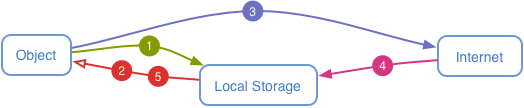
\includegraphics[width=4in]{figures/atmos-02.png}
  \caption{Overview of Atmosphere functioning}
  \label{fig:figures_atmos-02}
\end{figure}

\begin{enumerate}
\item Object is saved to local storage. 
\item User interface is immediately updated
\item Request is made to update the object on the remote side
\item Local version is updated from the response
\item User interface is updated according to changes received from the server
\end{enumerate}

\subsubsection{API Example}

\begin{lstlisting}[caption=Fetching objects from remote source,label=list1]
MyModel.sync(remote: true)
\end{lstlisting}

Code in Listing \ref{list1} fetches remote data and persists them in a local collection. Triggers an event on the model, so that the user interface could be updated.

\begin{lstlisting}[caption=Saving object,label=list2]
myRecord.save(remote: true)
\end{lstlisting}
    
Code in Listing \ref{list2} stores changes in local storage and makes remote request. When the request is done, it updates the local data and triggers event to update the user interface.

\subsubsection{Features}

\begin{enumerate}
\item \textbf{API configuration}: Advanced options of configuring API. So far used with typical Rails app and Google Tasks API.
\item \textbf{Fetching and caching}: Objects can be fetched and cached in local storage.
\item \textbf{Sync and posting}: When object is changed, it's saved locally, then posted to the server.
\item \textbf{Offline usage}: The design allows for building offline applications.
\item \textbf{Live updating}: Comes with [atmos2-server](https://github.com/vojto/atmos2-server) which is lightweight Node.js proxy for updating objects in real time.
\end{enumerate}

\subsubsection{Notes}

The current implementation uses the model layer of \href{http://spinejs.com}{Spine.js}. All the code that works with Spine is encapsulated in the AppContext class, which is 80 lines of CoffeeScript.

\subsection{Getting started with the JavaScript library}

Take existing Spine app or create a new one.

Install atmos2.

\begin{lstlisting}[caption=Installing atmos2 package]
git clone git://github.com/vojto/atmos2.git node_modules/atmos2
\end{lstlisting}

\textbf{Adding modules to slug.json}

Add these modules to your \texttt{slug.json}:

\begin{lstlisting}[caption=Updating slug.json with atmos2 package]
"dependencies": [
…
	"atmos2",
	"atmos2/lib/spine"
],
\end{lstlisting}

\textbf{Setting up the model}

Let's say this is your current Spine model:

\begin{lstlisting}[caption=Current Spine model]
class Task extends Spine.Model
  @configure 'Task', 'title', 'kind', 'selfLink'
\end{lstlisting}

\textbf{Extending the model}

All you have to do is require Atmosphere's Spine adapter, and extend model with it.

\begin{lstlisting}[caption=Requiring Atmosphere's Spine adpater]
require('atmos2/lib/spine')

class Task extends Spine.Model
  @configure 'Task', 'title', 'kind', 'selfLink'
  @extend Spine.Model.Atmosphere
\end{lstlisting}

Atmosphere will automatically use the local storage.

\textbf{Setting up the synchronizer}

Do this somewhere, where it will be executed before anything else.

\begin{lstlisting}[caption=Setting up the synchronizer]
Atmos = require('atmos2')

atmos = new Atmos
atmos.resourceClient.base = "https://www.googleapis.com/tasks/v1/users/@me"
\end{lstlisting}

As you can see, this example will work with Google Tasks API. But first, Atmosphere needs more information.

\begin{lstlisting}[caption=Setting up Synchronizer]
atmos.resourceClient.routes =
  Task:
    index: "/lists"
atmos.resourceClient.addHeader "Authorization", "OAuth #{token}"
atmos.resourceClient.IDField = "id"
atmos.resourceClient.dataCoding = "json"
atmos.resourceClient.itemsFromResult = (result) -> result.items
\end{lstlisting}
    
\begin{enumerate}
\item \texttt{routes} specifies path that will be hit on actions: index, create, update, delete. (TODO: Add others to the example.)
\item \texttt{addHeader} adds header to every request. In this case, we're adding OAuth Authorization, which we've taken care of someplace else, so we have a token.
\item \texttt{IDField} every retrieved object must have an ID. Some APIs expose this ID in field \texttt{id}, others \texttt{identifier}, so this settings lets you set it. If a record with empty ID will be retrieved, Atmosphere will throw an error.
\item \texttt{dataCoding} can be \texttt{form} or \texttt{json}, specifies in what format will be outgoing data encoding and sent. (Also, what \texttt{Content-Type} will be used)
\item \texttt{itemsFromResult} is a function that will be used to get the items from object decoded from response JSON. In this case, we receive a JSON that looks like this: \texttt{{items: [...]}}, so we need to tell Atmosphere how to look for actual records.
\end{enumerate}


\subsubsection{Fetching objects}

\begin{lstlisting}[caption=Fetching objects]
Task.sync(remote: true)
\end{lstlisting}

This will first fetch data from local storage triggering the \texttt{refresh} event, then make the network request, update local data, and trigger \texttt{refresh} event again.

\subsubsection{Saving objects}

\begin{lstlisting}[caption=Sending objects]
task = new Task({title: "Task 2"})
task.save(remote: true)
\end{lstlisting}

Calling \texttt{save} will first save the object locally, then it will make network request to save it again. \texttt{create} action will be used.

If you call \texttt{save} on already saved object, \texttt{update} action will be used. Atmosphere keeps track of all objects you saved with \texttt{remote} flag to differentiate between objects that have been sent previously and those once that haven't.

\subsection{Getting started with the Cocoa library}

\subsubsection{Installation}

Atmosphere for Cocoa is available as \href{http://cocoapods.org/}{CocoaPods} package. In order to install Atmosphere, your first need to enable CocoaPods for your project. For installation instructions please see the \href{http://cocoapods.org/}{CocoaPods} website.

Add Atmos2 to your Podfile.

\begin{lstlisting}[caption=Adding Atmos2 to your Podfile]
dependency 'Atmos2', {:git => 'git@github.com:vojto/atmos2-cocoa.git', :branch => 'master'}
\end{lstlisting}

\subsubsection{Setup}

The next step is to setup the synchronizer. In order to do that, open the main entry point for your application (usually the app delegate) and include Atmos2 header file.

\begin{lstlisting}[caption=Including Atmos2 header file]
#import <Atmos2/Atmosphere.h>
\end{lstlisting}

In your main class header file create a new instance variable that will hold reference to the synchronizer.

\begin{lstlisting}[caption=Adding instance variable for synchronizer]
@property (strong) ATSynchronizer *sync;
\end{lstlisting}

The next step is to set up the synchronizer.

\begin{lstlisting}[caption=Setting up the synchronizer, label=lst3]
self.sync = [[ATSynchronizer alloc] initWithAppContext:self.managedObjectContext];
[self.sync setBaseURL:@"http://localhost:6001"];
[self.sync loadRoutesFromResource:@"Routes"];
[self.sync setIDField:@"_id"];
\end{lstlisting}

The Listing \ref{lst3} shows very simple setup that first initializes a new synchronizer with current application context, sets base URL of the REST source, loads routing table from \texttt{Routes.plist} and finally sets up the ID field for parsing responses.

The routes file should contain a dictionary for each entity with keys representing actions and values representing HTTP actions in \texttt{method /path} format. An example routes file is portrayed in Figure \ref{fig:figures_routes-cocoa}.

\begin{figure}[htbp]
  \centering
    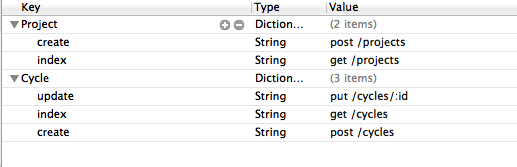
\includegraphics[width=4in]{figures/routes-cocoa.png}
  \caption{Example routes file}
  \label{fig:figures_routes-cocoa}
\end{figure}

\subsubsection{Fetching objects}

Listing \ref{lst4} shows how to fetch objects for an entity Project.

\begin{lstlisting}[caption=Fetching objects for an entity,label=lst4]
[self.sync fetchEntity:@"Project"];
\end{lstlisting}

Calling this command will fetch remote objects and store them locally. The application should be using data bindings or similar mechanism to update data when they change in Core Data store.

\subsubsection{Saving objects}

Saving objects is done automatically by watching changes in Core Data context. When an object is saved locally such as code in Listing \ref{lst5} shows, Atmosphere automatically sends it to the server.

\begin{lstlisting}[caption=Saving objects locally,label=lst5]
PLProject *project = (PLProject *)[NSEntityDescription insertNewObjectForEntityForName:@"Project" inManagedObjectContext:self.context];
project.title = @"New Project";
[self.context save:&error];
\end{lstlisting}
%
%
% \ititnclude{appendixc}
%% begin the 'Curriculumvitae' of the author
% \curriculumvitae\protect\label{page:posledna}
% Táto časť\/ je nepovinná. Autor tu môže uviesť\/ svoje biografické
% údaje, údaje o~záujmoch, účasti na~projektoch, účasti na~súťažiach,
% získané ocenenia, zahraničné pobyty na~praxi, domácu prax, publikácie
% a~pod.
% \endcurriculumvitae

\end{document}
%%